\begin{titlepage}

\begin{figure}[H]
  \begin{center}
    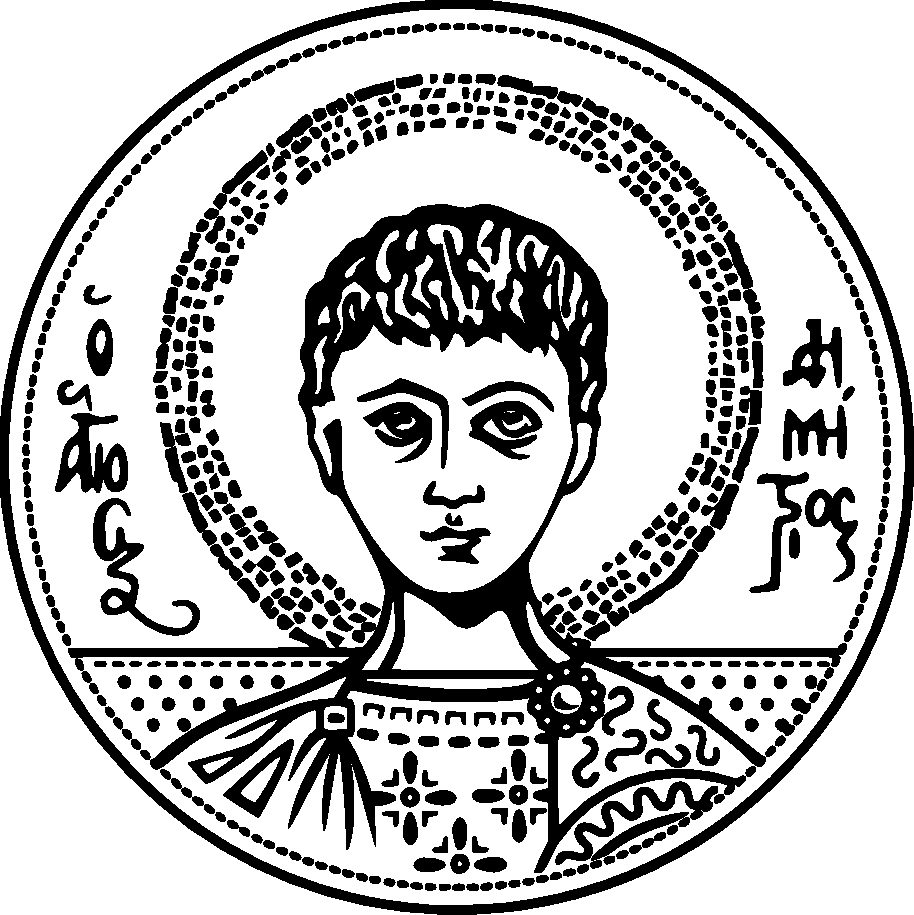
\includegraphics[width=3cm]{auth.pdf}
    \label{fig:cover_auth_logo}
  \end{center}
\end{figure}

\centering
\Large Αριστοτέλειο Πανεπιστήμιο Θεσσαλονίκης\\
\Large Πολυτεχνική Σχολή\\
\large Τμήμα Ηλεκτρολόγων Μηχανικών και Μηχανικών Υπολογιστών\\
\large Τομέας Ηλεκτρονικής και Υπολογιστών

\vspace{\fill}

\LARGE Υπολογισμός της Ευκλείδειας Απόστασης δύο Τριγωνικών Πλεγμάτων

\vspace{\fill}

\Large Διπλωματική Εργασία\\
\Large Καρελής Παναγιώτης

\vspace{\fill}
\raggedright

\begin{tabular}{ll}
\textbf{Επιβλέπων:} & Πιτσιάνης Νικόλαος\\
 & Αναπληρωτής Καθηγητής Α.Π.Θ.\\
\end{tabular}

\centering
\vspace{\fill}
\today

\end{titlepage}

\begin{abstract}
Σε μια πληθώρα εφαρμογών της Υπολογιστικής Γεωμετρίας 
(Μηχανική με τη Βοήθεια Υπολογιστών (\tl{CAE}), Προσομοιώσεις με Υπολογιστές, 
Ρομποτική, Γραφική με Υπολογιστές κ.α.)
τα αντικείμενα του χώρου αναπαρίστανται συνήθως από 
πολυγωνικά πλέγματα.
Κοινό πρόβλημα για όλους τους παραπάνω τομείς αποτελεί η εύρεση της
απόστασης που διαχωρίζει δύο αντικείμενα και η ανίχνευση σύγκρουσης
μεταξύ τους.
Στην παρούσα εργασία, προτείνουμε αποδοτικούς αλγορίθμους που υπολογίζουν 
την Ευκλείδεια απόσταση δύο αντικειμένων του τρισδιάστατου χώρου και τους υλοποιούμε 
για την περίπτωση των τριγωνικών πλεγμάτων. 
Για τους αλγορίθμους αυτούς σχεδιάζουμε μια δενδρική δομή δεδομένων που
ανήκει στην κατηγορία των Ιεραρχιών Οριoθετικών Όγκων (\tl{BVH}).
Η διαδικασία κατασκευής της παραπάνω δομής είναι παρόμοια με αυτή
του \tl{KD-Tree}, με τη διαφορά ότι η δομή μας διαχειρίζεται
χωρικά δεδομένα και κάνει χρήση 
Οριοθετικών Πλαισίων Ευθυγραμμισμένων με τους Άξονες (\tl{AABB}). 
Επιπλέον, περιγράφουμε έναν τρόπο διάσχισης της δομής ώστε να
υποστηρίζει ερωτήματα κοντινότερου γείτονα για χωρικά δεδομένα.
Η διάσχιση της δενδρικής δομής σχεδιάζεται ως μια κατευθυνόμενη 
αναζήτηση κατά βάθος (\tl{DFS}), που στοχεύει στη σμίκρυνση του 
χώρου αναζήτησης μέσω κλαδέματος του δένδρου κατά την 
οπισθοδρόμηση. 
Ακόμη, στην υλοποίηση μας παραλληλοποιούμε τη διαδικασία
κατασκευής του δένδρου όπως και τη διαδικασία αναζήτησης της ελάχιστης 
απόστασης κάνοντας χρήση πολλαπλών νημάτων επεξεργασίας. 
Τέλος, μετράμε και αναλύουμε την επίδοση των αλγορίθμων μας σε μια σειρά
από περιπτώσεις ελέγχου που κατασκευάσαμε. 

\textbf{Λέξεις-κλειδιά:} \\
\textit{Υπολογιστική Γεωμετρία, Πολυγωνικά Πλέγματα, Ευκλείδεια Απόσταση,
Ιεραρχίες Οριοθετικών Όγκων}
\end{abstract}

\selectlanguage{english}
\begin{abstract}
In a plethora of fields in Computational Geometry 
(Computer Aided Engineering, Computer Simulations,
Robotics, Computer Graphics etc.) objects in space are 
represented as polygonal meshes.
A common problem, for all the above, is the computation of
separation distance and collision detection of two objects.
In this thesis, we propose efficient algorithms that compute 
the Euclidean distance of two objects in 3D space and we implement
them for the case of triangle meshes.
For these algorithms we design a tree data structure that 
belongs to the family of Bounding Volume Hierarchies (BVH).
The construction procedure of this data structure is similar
to the one used by the KD-Tree, but it differs, as our data 
structure manages spatial data and also uses Axis-Aligned 
Bounding Boxes (AABB).
In addition, we describe a traversal scheme of the data 
structure in order to answer nearest neighbor queries 
for spatial data.
The traversal of the tree structure is implemented 
as a directed depth first search (DFS), aiming to reduce 
the searching space by pruning the tree during backtracking.
Furthermore, we parallelize the construction of the data 
structure as well as the procedure of finding the Euclidean
distance, using multithreading.
Finally, we measure and analyze the efficiency of our 
algorithms on a series of test cases we created.

\textbf{Keywords:} \\
\textit{Computational Geometry, Polygonal Meshes, Euclidean Distance,
Bounding Volumes Hierarchies}

\end{abstract}

\thispagestyle{empty}

\selectlanguage{greek}

\section*{Ευχαριστίες}
\thispagestyle{empty}

Με την παρούσα διπλωματική εργασία ολοκληρώνω τις σπουδές μου 
στο τμήμα Ηλεκτρολόγων Μηχανικών και Μηχανικών Η/Υ του Α.Π.Θ. 
Θα ήθελα να ευχαριστήσω τον καθηγητή μου Νικόλαο Πιτσιάνη 
όχι μόνο για τις γνώσεις που μου παρείχε αυτά τα χρόνια, αλλά 
και για την καταλυτική συνδρομή του στο να ανακαλύψω τα ενδιαφέροντα 
μου μέσα στο ευρύ φάσμα δραστηριοτήτων ενός μηχανικού υπολογιστών.

Ευχαριστώ τους γονείς μου Βασίλη και Νίκη καθώς και την αδερφή μου 
Δήμητρα, για τη συμπαράσταση τους σε όλο αυτό το ταξίδι και για την εμπιστοσύνη 
που μου έδειξαν από την πρώτη στιγμή.

Πολλά ευχαριστώ στον φίλο μου, και συνάδελφο, Μανώλη, που με βοήθησε να 
εξελιχθώ σε όλους τους τομείς της ζωής μου.

Ευχαριστώ την οικογένεια Καραγεωργίου, η οποία στάθηκε δίπλα μου σαν 
δεύτερη οικογένεια.
Ιδιαίτερα ευχαριστώ τον Λάζαρο και τον Ιωσήφ, που με τον τρόπο τους, 
με βοήθησαν να βελτιωθώ και έπαιξαν σημαντικό ρόλο στις αποφάσεις 
που πήρα μέχρι τώρα και στις αποφάσεις που θα πάρω στο μέλλον.

Τέλος, ευχαριστώ όλους τους φίλους, συναδέλφους και γνωστούς που πέρασα 
μαζί τους στιγμές τις οποίες θα θυμάμαι για πάντα,
όταν θα σκέφτομαι τα φοιτητικά μου χρόνια.


\clearpage
